\section{Data acquisition}
\label{sec:data_acquisition}

In our project, we capture different data streams. Our main mode of data acquisition is video streams from RGBD cameras. With RGBD cameras, as the name suggests, we capture two different modalities, RGB data and depth data. RGBD was discussed in section \ref{sec:rgbd_cameras}. In addition to the RGBD data, we also capture the human pose data from the Nuitrack system. The data acquisition is done using the Nuitrack SDK. The Nuitrack SDK is a software development kit that allows us to capture data from the Nuitrack system. 3DiVi does not offer any white paper or documentation on how their method works exactly. However, they have informed us that they use a CNN to estimate the pose of a human and that this CNN uses both RGB and depth information to estimate the pose of a human. 

Additionally to the pose data, the Nuitrack SDK allows us to capture the data from the RGBD cameras. This provides us with inherently synchronized data from the RGBD cameras and the pose data. An example of a pose can be seen in Figure \ref{fig:nui_skeleton}.

\begin{figure}
    \centering
    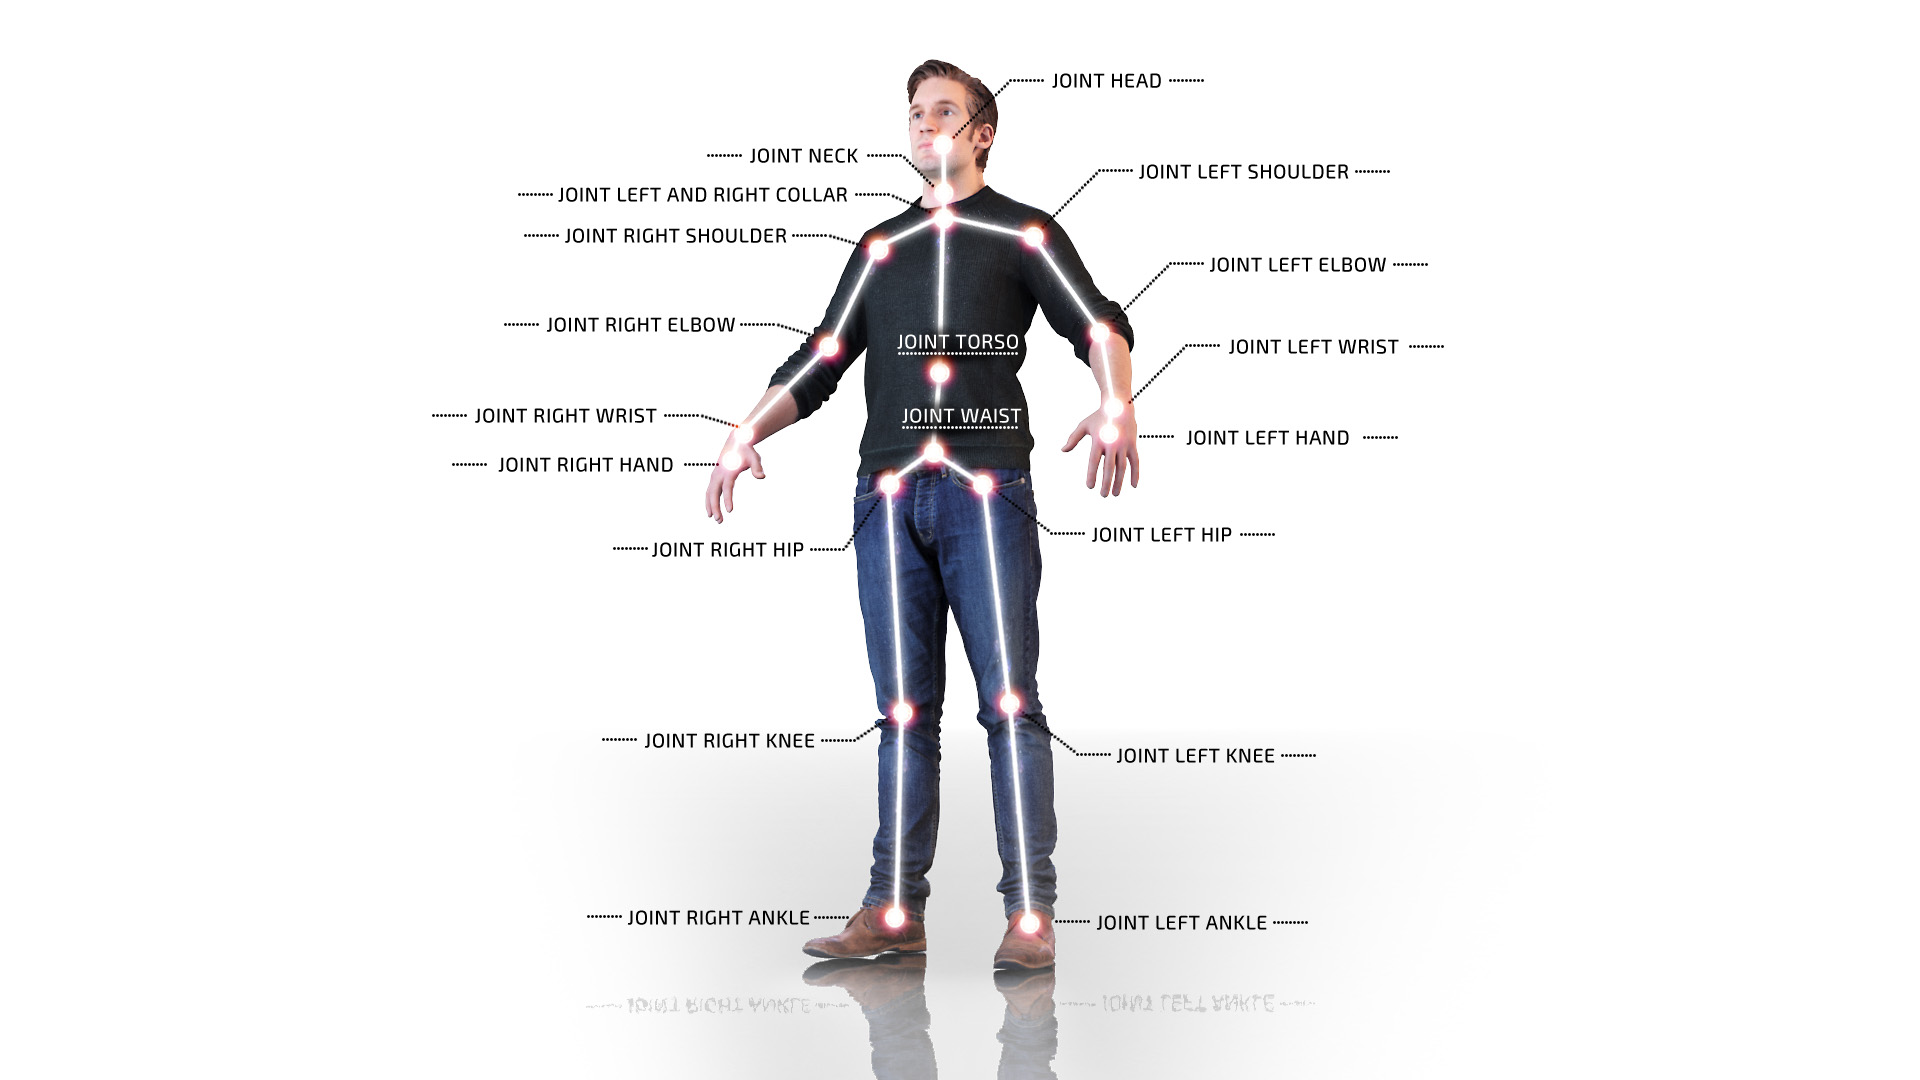
\includegraphics[width=\linewidth]{figures/HPE/Nui_skeleton_scheme.jpg}
    \caption[Nuitrack skeleton scheme]{The skeleton scheme used by Nuitrack.}
    \label{fig:nui_skeleton}
\end{figure}

Once the visual data is acquired from any stream there are only limited options to optimise the data. The most important aspect of this is the frames per second. Once a stream is recorded at a certain framerate, it is not possible to change this, except for duplicating or interpolating frames, which do not offer a high-quality result. Therefore, it is important to ensure that the frames can be recorded at a high enough rate. In a lot of cases, the first thought might be to record and query frames asynchronously but with asynchronous data acquisition the question of synchronisation arises. This is especially true if the data is recorded from multiple streams.

To maximise the frame rate, we limit any overhead that might be introduced by the data acquisition process. During the recording, we do not store the frames to file but instead, store the raw frames in memory to store them in the file later on. This reduces the overhead of writing to files and it is viable since we can manually limit the frames that are recorded for each recording beforehand to avoid any slow down due to memory limitations.
